%%%%%%%%% JPS abstruct %%%%%%%%%%%%%%%%%%%%%%%%%%%%%%%%%%%%%%%%%%
\documentclass[12pt,a4paper,dvipdfmx]{jsarticle}

%%%%%%%%% packages %%%%%%%%%%%%%%%%%%%%%%%%%%%%%%%%%%%%%%%%%%%%%%
\usepackage{graphicx} % Include figure files
\usepackage{wrapfig}		% 図の周りに本文を流し込みたいときに使用
\usepackage{subfigure}
\usepackage{here}
\usepackage[%                           % 余白の設定
%mag=1400,%                              jarticle の場合(14ptに)
truedimen,%
top=30truemm,bottom=20truemm,%
left=10truemm,right=10truemm]{geometry}
\pagestyle{empty}

%%%%%%%%% header %%%%%%%%%%%%%%%%%%%%%%%%%%%%%%%%%%%%%%%%%%%%%%%%
\begin{document}
\vspace{-5pt}
\begin{center}
{\gt \Large Mg-LPSOにおけるL1$_2$クラスターとスモールクラスターの相互作用}\\[10pt]

{\gt \large 関西学院大 理工 \\森下 慎也, 西谷 滋人}\\[5pt]

{\large \bf Interaction between L1$_2$ cluster and small cluster in Mg-LPSO}\\[5pt]

{\large \it Kwansei Gakuin Univ., Informatics.}\\ 

{\large \bf Shigeto R. Nishitani, Shinya Morishita}
\end{center}

\vspace{10pt}
%%%%%%%%% main %%%%%%%%%%%%%%%%%%%%%%%%%%%%%%%%%%%%%%%%%%%%%%%%%%
\paragraph{背景}
我々はMg-LPSO合金におけるLPSO構造の生成機構について,
「積層欠陥部に$L1_2$クラスターが形成され,そこから排斥されたZn, Yが濃化して新たな積層欠陥を誘発する」という仮説を立てていた\cite{sakamoto}.
これまでの研究では,L1$_2$クラスターと溶質原子単体,あるいはペアとの相互作用を調べるために,L1$_2$クラスターから一層ずつ離れた位置に溶質原子を挿入したモデルのエネルギーを第一原理計算により求めた結果は,溶質原子がL1$_2$クラスターから離れれば離れるほど安定化するという結果であった.
しかし,この結果に基づいた組織の発展シミュレーションでは,溶質原子の中距離秩序が現れない.
そこで,本研究ではより大きな溶質原子のクラスター集合を仮定し,第一原理計算によりL1$_2$クラスターとの相互作用エネルギーを求めた.
\begin{wrapfigure}{r}{5cm}
\vspace{-1.4\baselineskip}
\begin{center}
   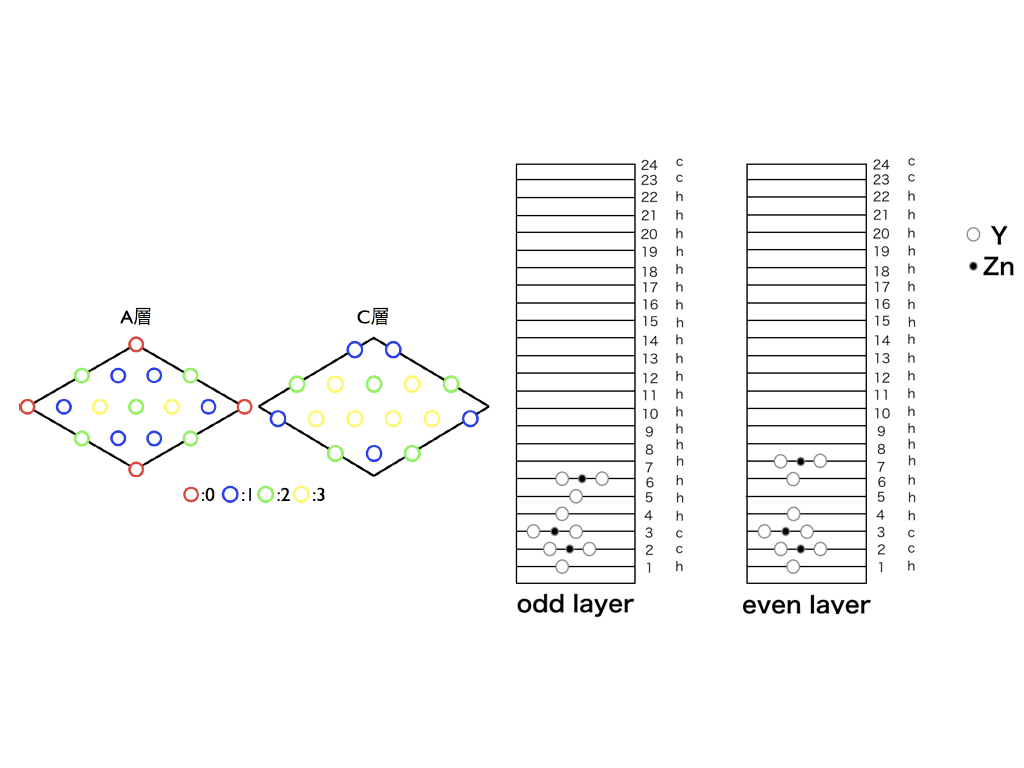
\includegraphics[width=50mm]{slab24_color.jpeg}
  \caption{A層とC層における近接距離を表した図と今回使用したスラブモデルの模式図.}
  \label{fig:one}
\end{center}
\vspace{-1\baselineskip}
\end{wrapfigure}
\vspace{-1\baselineskip}
\paragraph{手法}
清原らはhcp構造にL1$_2$クラスターを導入すると,構造緩和により上下分割されスモールクラスターが生成されると報告していた\cite{kiyohara}.このスモールクラスターに着目し,図\ref{fig:one}に示すスラブモデルに挿入し系全体のエネルギーを求めた.図\ref{fig:one}において同じ色で示した等価な位置へスモールクラスターを配置したモデルについて第一原理計算をおこなった.

\begin{wrapfigure}{r}{5cm}
\vspace{2\baselineskip}
\begin{center}
   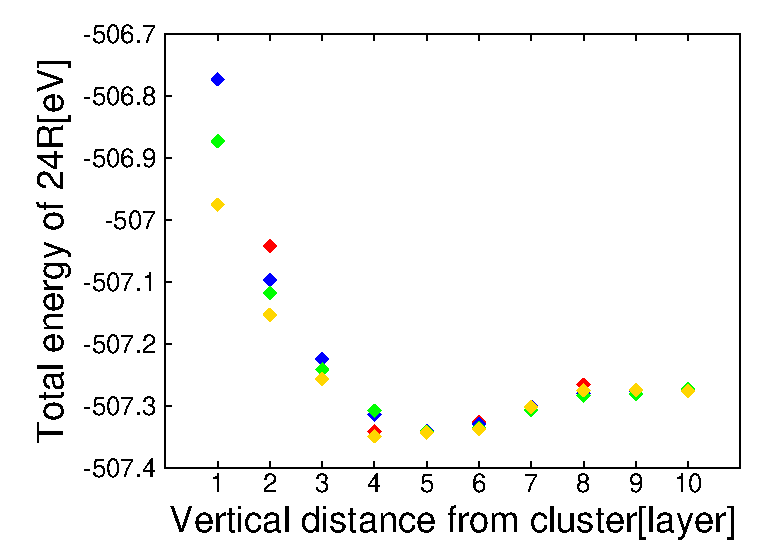
\includegraphics[width=50mm]{smallcluster_Alld_JPS2017.eps}
  \caption{$L1_2$クラスターとsmall clusterの距離によるエネルギー変化.グラフの点の色は図\ref{fig:one}で示した近接距離の色に対応している.}
  \label{fig:two}
\end{center}
\vspace{-1\baselineskip}
\end{wrapfigure}
\vspace{-1\baselineskip}


\paragraph{結果}
図\ref{fig:two}にL1$_2$クラスターとスモールクラスター間の垂直距離による系全体のエネルギーの変化を示した.エネルギー値は4-5層離れた位置で最低値となり,6層以上の距離でも単調に減少することなく,僅かではあるが中距離で溶質原子が安定する傾向を示している.エネルギー的に得られた中距離での安定性から,動的な組織形成機構を解明するためには,スモールクラスターの拡散機構について議論をおこなう必要がある.そこで,我々は単空孔,あるいは複空孔を利用した空孔拡散に着目し,スモールクラスター周辺での空孔の安定性について報告する.
\vspace{-0.5\baselineskip}
%%%%%%%%%%%%%%%%%%%%%%%%%%%% Figure 1 %%%%%%%%%%%%%%%%%%%%%%%%%%%%%%%%%%%%%
%\begin{figure}[h]
%\begin{center}
%\includegraphics[width=5cm]{JPS.eps}
%\end{center}
%\caption{日本物理学会のマーク。カラー図面が掲載できるようになった。 }
%\end{figure}
%%%%%%%%%%%%%%%%%%%%%%%%%%%%%%%%%%%%%%%%%%%%%%%%%%%%%%%%%%%%%%%%%%%%%%%%%%%


{\small\setlength\baselineskip{10pt}	% 参考文献は小さめの文字で行間を詰めてある
\begin{thebibliography}{9}
\bibitem{sakamoto}Y. Sakamoto, C. Shirayama, Y. Yamamoto, R. Kubo, M. Kiyohara, and S. R. Nishitani: Mater.Trans., 56(2015), 933.
\bibitem{kiyohara} M. Kiyohara, Y. Sakamoto, T. Yoshioka, S. Morishita, and S. R. Nishitani: proceedings of PRICM, (Kyoto 2016), to be publishedではないやろ?????.
%\bibitem{okuda}H. Okuda, M. Yamasaki, Y. Kawamura, M. Tabuchi, H. Kimizuka: Scientific Reports 5 (2015), 14186.
\end{thebibliography}
}


\end{document}
